%!TEX TS-program = LuaLaTeX
\documentclass[tikz,border=0.5cm]{standalone}

\pdfvariable suppressoptionalinfo \numexpr32+64+512\relax

\begin{document}
 % without matrix library
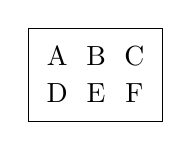
\begin{tikzpicture}
\node[matrix,draw]{
\node(a){A}; & \node(b){B}; & \node(c){C}; \\
\node(d){D}; & \node(e){E}; & \node(f){F}; \\
};
\end{tikzpicture}
\end{document}
 

 